\nonstopmode
%==============================================================================
%== template for LATEX poster =================================================
%==============================================================================
%
%--A0 beamer slide-------------------------------------------------------------
\documentclass[final]{beamer}

\usepackage{graphicx}
\usepackage{xcolor}
\usepackage[orientation=portrait,size=a0,
            scale=2.2         % font scale factor
           ]{beamerposter}
           
\geometry{
  hmargin=2.5cm, % little modification of margins
}

%
\usepackage[utf8]{inputenc}
\usepackage{ragged2e}

\linespread{1.15}
%
%==The poster style============================================================
\usetheme{sharelatexback}

%==Title, date and authors of the poster=======================================
%\title
%[http://python.fossee.in, info@fossee.in, python@fossee%.in] % Conference
%{ % Poster title
%}


%\author{ % Authors
%Author One\inst{1}, Author Two\inst{2}, Author Three\inst{2,3}
%}
%\institute
%[Very Large University] % General University
%{
%\inst{1} Very Large University, Neverland
%\inst{2} Other University, Neverland
%\inst{3} Yet Another University, Neverland
%}
%\date{\today}



\begin{document}
\begin{frame}[t]
%==============================================================================
\begin{multicols}{2}
%==============================================================================
%==The poster content==========================================================
%==============================================================================

%% BACK

\section{How can you learn Python ?}
\begin{itemize}
\item \justifying {{\bf{Spoken Tutorial}} - The FOSSEE project has created a series of Spoken Tutorials on
Python.  These are available for learning, on the Spoken Tutorial
website, free of cost. You can access these tutorials from this link:
{\color{blue}python.fossee.in/spoken-tutorials}} \par

\vskip5ex

\begin{figure}
\centering
\fboxsep=0mm%padding thickness
\fboxrule=1pt%border thickness
\fcolorbox{gray}{white}{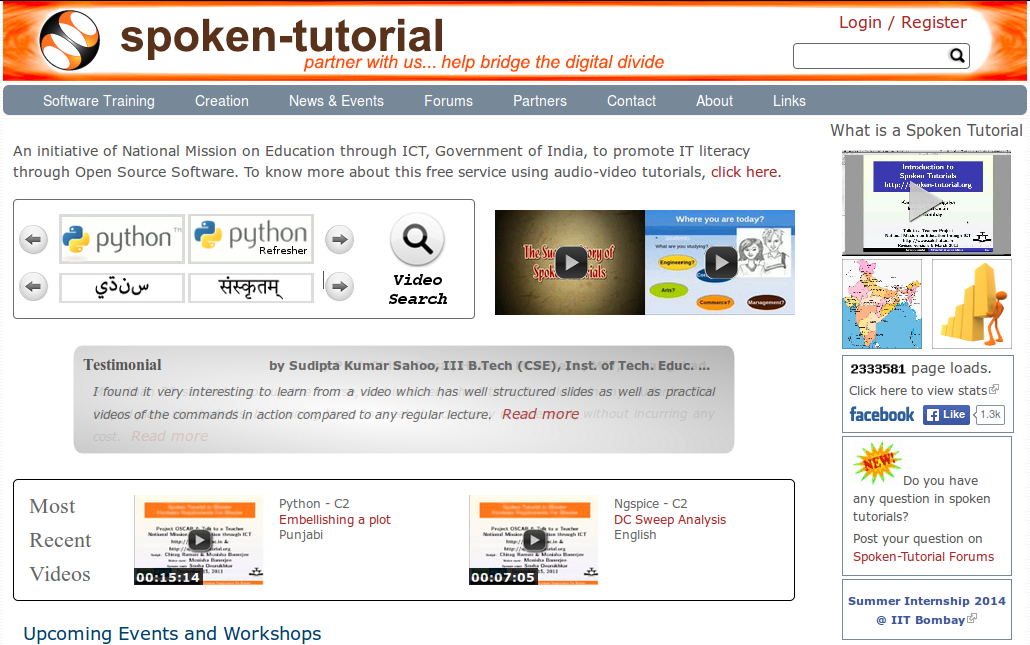
\includegraphics[width=0.9\columnwidth]{st.png}}
\texttt{\small Spoken Tutorial website}
%\caption{Spoken tutorial website}
\end{figure}

\vskip5ex

\item \justifying{{\bf{Textbook Companion Internship}} - Learn Python
  in a practical way by contributing to the Python Textbook Companion
  Internship. It aims to create Companions by coding solved examples
  from Standard textbooks using Python. Participate and earn
  attractive honorarium and Certificate of Internship from FOSSEE, IIT
  Bombay!  For more details, please visit: \\
  {\color{blue}python.fossee.in/textbook-companion-project}}\par

\vskip5ex

\begin{figure}
\centering
\fboxsep=0mm%padding thickness
\fboxrule=1pt%border thickness
\fcolorbox{gray}{white}{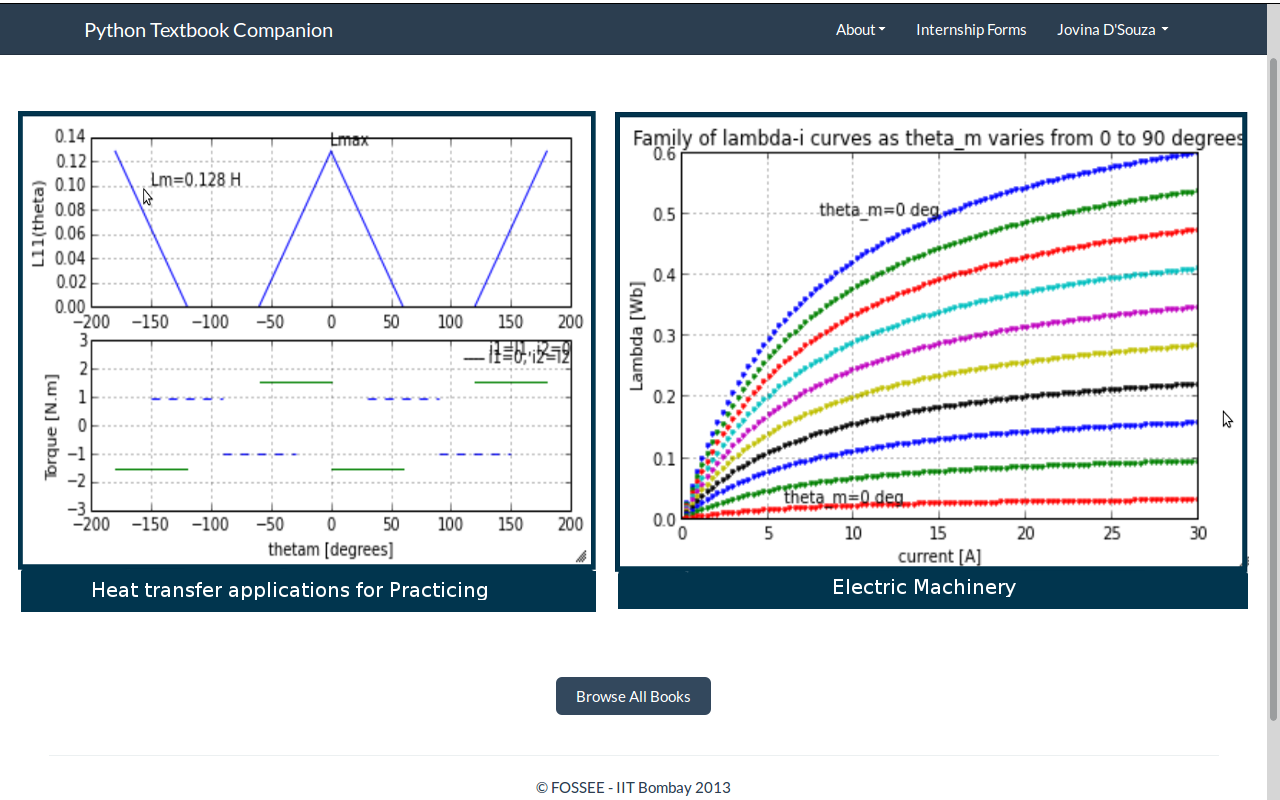
\includegraphics[width=0.9\columnwidth]{tbc.png}}
\texttt{\small Python Textbook Companion website}
%\caption{Python textbook companion}
\end{figure}


\vskip5ex

\item {{\bf{SELF Workshops}} - The Spoken Tutorial Team conducts
  workshops on Python.  These work- shops are completely free of cost
  and are conducted without the need of any domain expert. Learn
  Python and obtain a certificate from Spoken Tutorial Project, IIT
  Bombay, upon successful completion of the post-workshop evaluation
  test. Please visit: {\color{blue}python.fossee.in/spoken-tutorials}}
\end{itemize}
  \vskip5ex  


\section{About us}
\subsection{Website:}
\begin{center}
{\color{blue}http://python.fossee.in}
\end{center}  

\section{Contact us}

\subsection{General help \& Queries:}
\begin{center}
info@fossee.in \\
python@fossee.in
\end{center}



%==============================================================================
%==End of content==============================================================
%==============================================================================
%--References------------------------------------------------------------------
%--End of references-----------------------------------------------------------

\end{multicols}

%==============================================================================
\end{frame}
\end{document}
